
\chapter{Detailed Kernel Descriptions}

\section{Intro}
In this chapter, architecture of each kernel is described in details, neglecting implementation aspect of it, like SLR or DDR bank assignments.

\pagebreak

\section{Concat2}
Concatenates two tensors of rank four into one over a dimension.
\subsection{Top Function}
\begin{lstlisting}
void task_concat(
		float* inputTn1,
	    float* inputTn2,
	    float* outputTn,

		unsigned int dimA0,
		unsigned int dimA1,
		unsigned int dimA2,
		unsigned int dimA3,

		unsigned int dimB0,
		unsigned int dimB1,
		unsigned int dimB2,
		unsigned int dimB3)
\end{lstlisting}

\subsection{Usage}
Concat Over Dim: 3
\vspace{0.5cm}
\begin{table}[htbp] % put table at (h:here, t:top, b:bottom, p:seperated page)
\caption{Usage Instances and Tensor Shapes}
\label{tab:shapes_concat}
	\begin{center}
		\begin{tabular}{|r|c|c|c|c|} 
		\hline	
		Tensor & Dim0 & Dim1 & Dim2 & Dim3\\ 
		\hline	
		InputTn1 &
			5 &
			1024 &
			1, 20 &
			3, 64, 128, 192 \\ 
		\hline
		InputTn2 &
			5 & 
			1024 & 
			1, 20 & 
			3, 64, 128 \\
		\hline
		OutputTn &
			Dim0 & 
			Dim1 & 
			Dim2 & 
			DimA3+DimB3 \\
		\hline
		\end{tabular}
	\end{center}
\end{table}

\subsection{Fixed Shape Instances}
\begin{table}[htbp] % put table at (h:here, t:top, b:bottom, p:seperated page)
\caption{Fixed Shaped Instances of Kernel Template}
\label{tab:shapes_concat}
	\begin{center}
		\begin{tabular}{|r|c|} 
		\hline	
		  & Instance 1\\ 
		\hline	
		DimA0 &
			5 \\ 
		\hline
		DimA1 & 
			1024\\
		\hline
		DimB0 & 
			5\\
		\hline
		DimB1 & 
			1024\\
		\hline
		\end{tabular}
	\end{center}
\end{table}

\subsection{Technical Details}
\begin{enumerate}
\item sadasd
\end{enumerate}


\pagebreak





\section{Sqrt}
Takes second root of each element in the input tensor of any rank.

\subsection{Top Function}
\begin{lstlisting}
void task_sqrt(
        float* inputTn,
        float* outputTn,
        unsigned long len)
\end{lstlisting}

\subsection{Usage}
Not available.

\subsection{Fixed Shape Instances}
None.

\subsection{Technical Details}
\begin{enumerate}
\item sadasd
\end{enumerate}






\pagebreak






\section{ReduceMax}
A reduction kernel with \textit{max} operator reducing on the element over the given dimension. The kernel is designed to operate on tensors of \textbf{rank three} for simplicity but it takes tensors of \textbf{rank four} in the usage cases as it is described below.
\subsection{Top Function}
\begin{lstlisting}
void task_reducemax(
        float* inputTn,
        float* outputTn,
		const unsigned int dim0,
		const unsigned int dim1,
		const unsigned int dim2,
		const int overaxis0,
		const int overaxis1,
		const int overaxis2)
\end{lstlisting}

\subsection{Usage}
Combination: FTF
\vspace{0.5cm}
\begin{table}[htbp] % put table at (h:here, t:top, b:bottom, p:seperated page)
\caption{Usage Instances and Tensor Shapes}
	\begin{center}
		\begin{tabular}{|r|c|c|c|c|} 
		\hline	
		Tensor & Dim0 & Dim1 & Dim2 & Dim3\\ 
		\hline	
		InputTn with reduction dim of 1 &
			5 &
			1024 &
			1 &
			1024 \\ 
		\hline	
		InputTn with reduction dim of 2 &
			5 &
			1024 &
			20 &
			64, 128 \\ 
		\hline
		\end{tabular}
	\end{center}
\end{table}

\begin{table}[htbp] % put table at (h:here, t:top, b:bottom, p:seperated page)
\caption{Kernel inputs for given usage instances}
	\begin{center}
		\begin{tabular}{|r|c|c|c|c|} 
		\hline	
		Reduction Dim & Arg Dim0 & Arg Dim1 & Arg Dim2 & Condition\\ 
		\hline	
		1 &
			Dim0 &
			Dim1 &
			Dim3 &
			Dim2=1 \\ 
		\hline	
		2 &
			Dim0*Dim1 &
			Dim2 &
			Dim3 &
			None \\ 
		\hline
		\end{tabular}
	\end{center}
\end{table}

\subsection{Fixed Shape Instances}
None.

\subsection{Technical Details}
\begin{enumerate}
\item sadasd
\end{enumerate}






\pagebreak






\section{Reduce Sum 4D}
A reduction kernel with summation operator, reducing elements of a four dimensional input tensor.
\subsection{Top Function}
\begin{lstlisting}
void task_reducesum4d(
        const float* inputTn,
        float* outputTn,
        const int pow_y,
        const unsigned int dim0,
        const unsigned int dim1,
        const unsigned int dim2,
        const unsigned int dim3,
        const int overaxis0,
        const int overaxis1,
        const int overaxis2,
        const int overaxis3)
\end{lstlisting}

\subsection{Usage}
Reduction Over Dim: 0,1,2 (TTTF)
\vspace{0.5cm}
\begin{table}[htbp] % put table at (h:here, t:top, b:bottom, p:seperated page)
\caption{Usage Instances and Tensor Shapes}
\label{tab:shapes_concat}
	\begin{center}
		\begin{tabular}{|r|c|c|c|c|} 
		\hline	
		Tensor & Dim0 & Dim1 & Dim2 & Dim3\\ 
		\hline	
		InputTn1 &
			5 &
			1024 &
			1, 20 &
			64, 128, 1024 \\ 
		\hline
		OutputTn &
			Dim3 & 
			 & 
			 & 
			 \\
		\hline
		\end{tabular}
	\end{center}
\end{table}

\subsection{Fixed Shape Instances}
None.

\subsection{Technical Details}
\begin{enumerate}
\item Pipelined loop with variable bound is used for moving data to and from global memory, because \emph{LOOP\_TRIPCOUNT} pragma could be used to estimate latency of the design. In contrast, it is not possible to add \emph{LOOP\_TRIPCOUNT} pragma for HLS \emph{memcpy(...)} with variable data length, meaning that latency estimation will not be available.

\item Unrolling a nested loop causes all of the sub-loops to be copied. For example if outermost loop has a trip count of four and it is completely unrolled, this means that there are four copies of any sub-loops in it.

\item A loop with burst read or write sub-loops can not be pipelined. Something like this.
\begin{lstlisting}
for(..){ // This loop can not be pipelined.
	for(..){//burst read
		..
	}
	
	for(..){//burst write
		..
	}
}
\end{lstlisting}

\item Unlike GPGPU, if-statements are favored in FPGA HLS. This is the reason of using a constant bound for-loop with a if-statement in the body of it, for checking the variable boundary.

\item For implementing \emph{pow\_y}, \emph{pow(..)} is not used, because the kernel does not require a floating point number as the power. Only the base is a floating point number. Using \emph{pow\_y} will result in higher latency.
\begin{lstlisting}
float pow_rslt = buff_tmp[i];
for(int ipwr=0;ipwr<(MAX_POW_Y_MINUS_ONE);ipwr++){
#pragma HLS UNROLL
	if(ipwr<pow_y_minus_one){
		pow_rslt = pow_rslt * pow_rslt;
	}
}
\end{lstlisting}

\item Three for-loops for \emph{dim0, dim1 and dim2} are fused together to decrease unnecessary latency of switching from one for-loop to another.

\item It might be a good idea to apply dataflow pragma in this kernel.

\end{enumerate}




\pagebreak









\section{Reduce Sum}
A reduction kernel with summation operator, reducing elements of a three dimensional input tensor.
\subsection{Top Function}
\begin{lstlisting}
void task_reducesum(
        const float * inputTn,
        float * outputTn,
        const unsigned int dim0,
        const unsigned int dim1,
        const unsigned int dim2,
        const int overaxis0,
        const int overaxis1,
        const int overaxis2)
\end{lstlisting}

\subsection{Usage}
Reduction Over Dim: 2 (FFT)
\vspace{0.5cm}
\begin{table}[htbp] % put table at (h:here, t:top, b:bottom, p:seperated page)
\caption{Usage Instances and Tensor Shapes}
\label{tab:shapes_concat}
	\begin{center}
		\begin{tabular}{|r|c|c|c|} 
		\hline	
		Tensor & Dim0 & Dim1 & Dim2\\ 
		\hline	
		InputTn1 &
			5 &
			1024 &
			3, 64 \\ 
		\hline
		OutputTn &
			Dim0 & 
			Dim1 & 
				\\
		\hline
		\end{tabular}
	\end{center}
\end{table}

\subsection{Fixed Shape Instances}
None.

\subsection{Technical Details}
\begin{enumerate}
\item This kernel also uses fused loops for \emph{dim0} and \emph{dim1}.

\item Fused loop is not pipelined, because it contains multiple sequential sub-loops.

\item Each slice of dim2 is read in burst mode and then processed by reduction sub-loop.

\item Different approaches have been tested for reduction sub-loop, details of each try and latency information is gathered in the following sub sections:

\subsubsection{Bypass with No Reduction}
Latency = 0.8 M clk

\subsubsection{Simple For-loop Reduction}
Latency = 4.3 M clk
\begin{lstlisting}
for(int i = 1 ; i< CONFIG_SLICE_SIZE;i++){
    	buff[0] += buff[i];
}
\end{lstlisting}

\subsubsection{Interleaved Parallel Reduction}
Latency = 4.0 M clk \\
Local buffer is partition with cyclic mode and factor of \emph{(CONFIG\_SLICE\_SIZE/2)}.

\begin{lstlisting}
#define CONFIG_SLICE_SIZE 64
float buff[CONFIG_SLICE_SIZE];
#pragma HLS ARRAY_PARTITION variable=buff cyclic factor=32 dim=1

//Parallel Reduction - Interleaved Addressing with Cyclic Partitioning of Local Buffer
//Compare cached slice with reduced slice(buff_rslt)
LoopReduction :for(int s=CONFIG_SLICE_SIZE/2;s>0;s>>=1){
#pragma HLS PIPELINE
#pragma HLS LOOP_FLATTEN off
#pragma HLS DEPENDENCE variable=buff array inter RAW true
	LoopIteration:for(int i=0;i<CONFIG_SLICE_SIZE/2;i++){
#pragma HLS LOOP_FLATTEN off
#pragma HLS UNROLL
#pragma HLS DEPENDENCE variable=buff array inter RAW false

		if(i<s){
			buff[i] += buff[i+s];
		}

	}
}
\end{lstlisting}

\subsubsection{Simple For-loop Reduction with Dataflow Pragma}
Latency = 3.3 M clk \\
For reduction, simple pipelined for-loop with II=10 is used.\\
Two outermost nested loops are not fused.
\begin{lstlisting}
    hls::stream<float> datastream1;
#pragma HLS STREAM variable=datastream1  depth=32
    hls::stream<float> datastream2;
#pragma HLS STREAM variable=datastream2  depth=32


LoopDim0: for(int d0=0; d0<dim0; d0++){
	LoopDim1: for(int d1=0; d1<dim1; d1++){
#pragma HLS DATAFLOW

		//Read 1 slice of dim2 from input tensor(burst read):
		SubfucSliceReadBurst(inputTn, datastream1, dim0, dim1, dim2, d0, d1);

		////Simple for-loop reduction
		SubfuncSliceReduceSum(datastream1,datastream2, dim2);

		//outputTn is of shape Dim0xDim1
		SubfuncSliceWrite(outputTn, datastream2, dim1, d0, d1);
	}
}

\end{lstlisting}

\end{enumerate}






\pagebreak






\section{MatOps}
Takes two input tensor and implements addition, subtraction, multiplication and division in a auto-tiling manner.
\subsection{Top Function}
\begin{lstlisting}
void task_matops(
		const float *inputTn1,
		const float *inputTn2,
		float * outputTn,
		const unsigned int dim0,
		const unsigned int dim1,
		const unsigned int dim2,
		const unsigned int dim3,
		const unsigned int dim0B,
		const unsigned int dim1B,
		const unsigned int dim2B,
		const unsigned int dim3B,
		const int dim0B_IsNotZero,
		const int dim1B_IsNotZero,
		const int dim2B_IsNotZero,
		const int dim3B_IsNotZero,
		const int mode)
\end{lstlisting}

\subsection{Usage}


\begin{table}[h]
\caption{Usage Instances and Tensor Shapes(Mode=0, Addition)}
\label{tab:shapes_matops}
	\begin{center}
		\begin{tabular}{|r|c|c|c|c|} 
		\hline	
		Tensor  & Dim0 & Dim1 & Dim2 & Dim3\\ 
		\hline	
		InputTn1 &
			5 &
			5,1024 &
			1,5,20,1024 &
			9,40,64,128,256,512,1024\\
		\hline	
		InputTn2 &
			 &
			5 &
			1024 &
			1,9,40,64,128,256,512,1024\\	
		\hline
		OutputTn &
			\multicolumn{4}{|c|}{Shape of InputTn1} \\
		\hline
		\end{tabular}
	\end{center}
\end{table}

\begin{table}[h]
\caption{Usage Instances and Tensor Shapes(Mode=1, Subtraction)}
\label{tab:shapes_matops}
	\begin{center}
		\begin{tabular}{|r|c|c|c|c|} 
		\hline	
		Tensor  & Dim0 & Dim1 & Dim2 & Dim3\\ 
		\hline	
		InputTn1 &
			5 &
			1024 &
			1,5,20 &
			3,64,128,256,512,1024\\
		\hline	
		InputTn2 &
			5 &
			1024 &
			20 &
			3,64,128,256,512,1024\\	
		\hline
		OutputTn &
			\multicolumn{4}{|c|}{Shape of InputTn1} \\
		\hline
		\end{tabular}
	\end{center}
\end{table}

\begin{table}[h]
\caption{Usage Instances and Tensor Shapes(Mode=2, Multiplication)}
\label{tab:shapes_matops}
	\begin{center}
		\begin{tabular}{|r|c|c|c|c|} 
		\hline	
		Tensor  & Dim0 & Dim1 & Dim2 & Dim3\\ 
		\hline	
		InputTn1 &
			5 &
			1024 &
			1,5,20,1024 &
			64,128,256,1024\\
		\hline	
		InputTn2 &
			 &
			 &
			 &
			1,64,128,256,1024\\	
		\hline
		OutputTn &
			\multicolumn{4}{|c|}{Shape of InputTn1} \\
		\hline
		\end{tabular}
	\end{center}
\end{table}

\begin{table}[htbp]
\caption{Usage Instances and Tensor Shapes(Mode=3, Division)}
\label{tab:shapes_matops}
	\begin{center}
		\begin{tabular}{|r|c|c|c|c|} 
		\hline	
		Tensor  & Dim0 & Dim1 & Dim2 & Dim3\\ 
		\hline	
		InputTn1 &
			5&
			1024&
			1,5,20&
			64,128,256,512,1024\\
		\hline	
		InputTn2 &
			&
			&
			&
			64,128,256,1024\\	
		\hline
		OutputTn &
			\multicolumn{4}{|c|}{Shape of InputTn1} \\
		\hline
		\end{tabular}
	\end{center}
\end{table}
\vspace{2 cm}
\subsection{Fixed Shape Instances}
None.

\subsection{Technical Details}
\begin{enumerate}
\item All four of the for-loops are fused together as a single loop to avoid unnecessary delays.
\item Fused loop is pipelined with II=1.
\end{enumerate}






\pagebreak





\section{ReLU}
Takes ReLU of input tensor of any shape.

\subsection{Top Function}
\begin{lstlisting}
void task_relu(
		const float *inputTn,
		float *outputTn,
		const unsigned long len)
\end{lstlisting}

\subsection{Usage}
\begin{table}[htbp] % put table at (h:here, t:top, b:bottom, p:seperated page)
\caption{Usage Instances and Tensor Shapes}
\label{tab:shapes_concat}
	\begin{center}
		\begin{tabular}{|r|c|c|c|c|} 
		\hline	
		Tensor & Dim0 & Dim1 & Dim2 & Dim3\\ 
		\hline	
		InputTn1 &
			5 &
			256,512,1024 &
			1,20 &
			64,128,1024 \\ 
		\hline
		OutputTn &
			Dim0 & 
			Dim1 & 
			Dim2 &
			Dim3	\\
		\hline
		\end{tabular}
	\end{center}
\end{table}

\subsection{Fixed Shape Instances}
None.

\subsection{Technical Details}
\begin{enumerate}
\item The for-loop is pipelined with II=1.
\end{enumerate}






\pagebreak





\section{Square}
Takes an input tensor of any shape and squares each element of it.

\subsection{Top Function}
\begin{lstlisting}
void task_square(
		const float * inputTn,
		float *outputTn,
		const unsigned long len)
\end{lstlisting}

\subsection{Usage}
\begin{table}[htbp] % put table at (h:here, t:top, b:bottom, p:seperated page)
\caption{Usage Instances and Tensor Shapes}
\label{tab:shapes_concat}
	\begin{center}
		\begin{tabular}{|r|c|c|c|c|} 
		\hline	
		Tensor & Dim0 & Dim1 & Dim2\\ 
		\hline	
		InputTn1 &
			5 &
			1024 &
			3,64\\ 
		\hline
		OutputTn &
			Dim0 & 
			Dim1 & 
			Dim2 \\
		\hline
		\end{tabular}
	\end{center}
\end{table}

\subsection{Fixed Shape Instances}
None.

\subsection{Technical Details}
\begin{enumerate}
\item The for-loop is pipelined with II=1.
\end{enumerate}










\pagebreak













\section{Tile}
Tiles the input tensor of rank three and four over the given dimension.

\subsection{Top Function}
\begin{lstlisting}
void task_tile(
		const float *inputTn,
		float *outputTn,
		unsigned int dim0,
		unsigned int dim1,
		unsigned int dim2,
		unsigned int dim3,
		unsigned int rank,
		unsigned int tileAxis,
		unsigned int tileCount)
\end{lstlisting}

\subsection{Usage}
\begin{table}[htbp] % put table at (h:here, t:top, b:bottom, p:seperated page)
\caption{Usage Instances and Tensor Shapes}
	\begin{center}
		\begin{tabular}{|r|c|c|c|c|c|} 
		\hline	
		Tensor & Dim0 & Dim1 & Dim2 & Dim3 & TileCount\\ 
		\hline	
		InputTn of Rank 3 and Tile Dim 1&
			5 &
			1 &
			1024 &
			  &
			1024\\ 
		\hline	
		InputTn of Rank 3 and Tile Dim 2&
			5 &
			1024 &
			1 &
			  &
			1024\\ 
		\hline 
		InputTn of Rank 4 and Tile Dim 2&
			5 &
			1024 &
			1 &
			3,64&
			20 \\ 
		\hline
		\end{tabular}
	\end{center}
\end{table}


\subsection{Fixed Shape Instances}
None.

\subsection{Technical Details}
\begin{enumerate}
\item Outermost for-loops are fused together.
\end{enumerate}












\pagebreak












\section{MatMul}
Batch matrix multiplication kernel. Takes two tensor of A and B of rank three as input and computes C=AB. Both matrices must be row-major and none should be transposed.

\subsection{Top Function}
\begin{lstlisting}
void task_matmul(
		int *inputTn1,
		int *inputTn2,
		int *outputTn,

		int dim0A,
		int dim1A,
		int dim2A,

		int dim0B,
		int dim1B,
		int dim2B)
\end{lstlisting}

\subsection{Usage}

\begin{table}[htbp] % put table at (h:here, t:top, b:bottom, p:seperated page)
\caption{Input tensor requirements}
\label{tab:shapes_concat}
	\begin{center}
		\begin{tabular}{|r|c|c|c|c|} 
		\hline	
		 & Dim0 & Dim1 & Dim2\\ 
		\hline	
		Matrix Data &
			Batch &
			Rows &
			Columns\\ 
		\hline 
		\end{tabular}
	\end{center}
\end{table}

\begin{table}[htbp] % put table at (h:here, t:top, b:bottom, p:seperated page)
\caption{Usage Instances and Tensor Shapes}
\label{tab:shapes_concat}
	\begin{center}
		\begin{tabular}{|r|c|c|c|c|} 
		\hline	
		Tensor & Dim0 & Dim1 & Dim2\\ 
		\hline	
		InputTn1 &
			1,5 &
			5,1024 &
			3,64,256,512,1024\\ 
		\hline
		InputTn2 &
			1,5 &
			3,64,256,512,1024 &
			3,9,40,256,512,1024\\ 
		\hline
		OutputTn &
			Dim0 & 
			Dim1A & 
			Dim2B \\
		\hline
		\end{tabular}
	\end{center}
\end{table}


\subsection{Fixed Shape Instances}
None.

\subsection{Technical Details}
\begin{enumerate}
\item The kernel uses tiled matrix multiplication approach which helps with non coalesced memory accesses for matrix B.
\item The basic operation of the kernel is illustrated in the figure \ref{fig:matmul01}.

\begin{figure}[h] 
\caption{MatMul Operation for Batch=1}
\label{fig:matmul01}
\centering
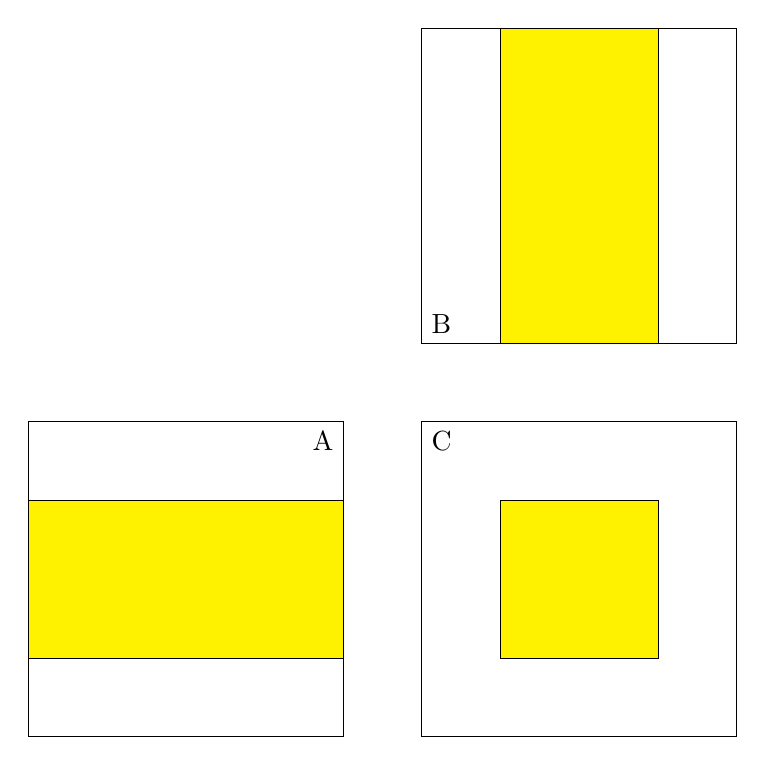
\begin{tikzpicture}
\draw [fill=yellow] 	(0,1) rectangle (4,3); 
\draw [fill=yellow] 	(6,1) rectangle (8,3); 
\draw [fill=yellow] 	(6,5) rectangle (8,9); 
\draw [] 	(0,0) rectangle (4,4);
\draw [] 	(5,0) rectangle (9,4);
\draw [] 	(5,5) rectangle (9,9);
\node [below left] at  (4,4) {A};
\node [below right] at (5,4) {C};
\node [above right] at (5,5) {B};
\dimline [color=cyan,extension start length=0.5 cm, extension end length=0.5 cm] {(0,4.5)}  {(4,4.5)}  {Common Dim}
\dimline [color=cyan,extension start length=0.5 cm, extension end length=0.5 cm] {(4.5,5)} {(4.5,9)} {Common Dim} 
\dimline [color=cyan,extension start length=0.5 cm, extension end length=0.5 cm] {(5,9.5)} {(9,9.5)} {Dim2B} 
\dimline [color=cyan,extension start length=0.5 cm, extension end length=0.5 cm] {(-0.5,0)} {(-0.5,4)} {Dim1A} 
\dimline [color=cyan,extension start length=-0.5 cm, extension end length=-0.5 cm] {(6,-0.5)} {(8,-0.5)} {Buffer\\Depth} 
\dimline [color=cyan,extension start length=-0.5 cm, extension end length=-0.5 cm] {(9.5,1)} {(9.5,3)} {Buffer\\Depth} 
\end{tikzpicture}
\end{figure}


\item It is important to note that in order to maximize performance it is essential to read elements of MatB less frequently, so the kernel will read the given tile of MatB once and hold it in the local buffer, then it will continuously read related tiles of MatA and compute output elements for given two local buffers of matrices A and B. 

\item According to \url{https://www.xilinx.com/support/answers/71596.html}, the memory banks for \emph{MatMul} kernel must be manually assigned by --sp option of the linker(XOCC). The option that is used is the following: \emph{--sp task\_matmul\_1.inputTn1:bank0 --sp task\_matmul\_1.inputTn2:bank0 --sp task\_matmul\_1.outputTn:bank0}
\end{enumerate}







\clearpage









\section{Transpose}
Takes an input tensor of rank three and performs batch matrix transpose operation on it. The input matrix should be row-major.

\subsection{Top Function}
\begin{lstlisting}
void task_transpose(
	const float* inputTn,
	float* outputTn,
	int dim0,
	int dim1,
	int dim2)
\end{lstlisting}

\subsection{Usage}
\begin{table}[htbp] % put table at (h:here, t:top, b:bottom, p:seperated page)
\caption{Usage Instances and Tensor Shapes}
\label{tab:shapes_transpose}
	\begin{center}
		\begin{tabular}{|r|c|c|c|c|} 
		\hline	
		Tensor & Dim0 & Dim1 & Dim2\\ 
		\hline	
		InputTn1 &
			5 &
			1024 &
			1,3,64\\ 
		\hline
		OutputTn &
			Dim0 & 
			Dim2 & 
			Dim1 \\
		\hline
		\end{tabular}
	\end{center}
\end{table}

\subsection{Fixed Shape Instances}
None.

\subsection{Technical Details}
\begin{enumerate}
\item The main idea behind the approach of the kernel is to minimize the latency that is in result of strided global memory accesses. This kernel reads and writes elements in a coalesced fashion. It uses the local buffer to facilitate the problem of high latency of the strided memory access for transposing operation.

\item (?) Possibly, to minimize the kernel's run-time, tile shape should be an square and size of this square should be as large as possible, but preferably(not necessarily) smaller than \emph{Min\{Dim1, Dim2\}}.

\item In the following figure, the arrows show the direction of memory r/w operations. The input and output are row-major arrays, So, horizontal arrows stand for coalesced memory accesses and vertical arrows stand for strided memory accesses.

\item In the figure, the middle square shows the local buffer.

\item For the HW-EMU mode, the memory banks for each one of the arguments of the kernel are manually set to bank 0.

\begin{figure}[h] 
\caption{Transposing Operation for inputTn of shape 1x4x4 and tile size of 2x2}
\label{fig:transpose01}
\centering
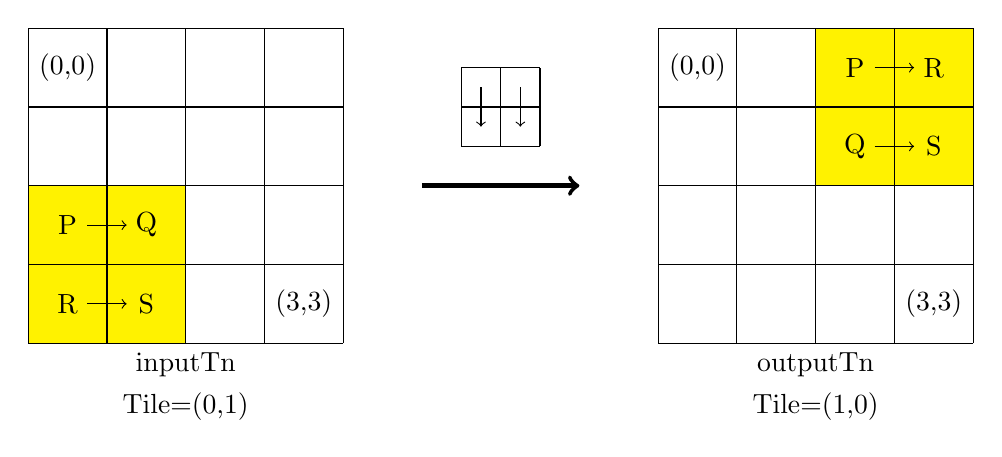
\begin{tikzpicture}
\draw [fill=yellow] 	(0,0) rectangle (2,2);  
\draw [] 	(0,0) grid (4,4); 
\node [below] at  (2,0) {inputTn}; 
\node [below] at  (2,-0.5) {Tile=(0,1)}; 

\node [] at  (0.5,1.5) {P}; 
\node [] at  (1.5,1.5) {Q}; 
\node [] at  (0.5,0.5) {R}; 
\node [] at  (1.5,0.5) {S}; 

\draw [->] (0.75,0.5) -- (1.25,0.5);
\draw [->] (0.75,1.5) -- (1.25,1.5);

\node [] at  (0.5,3.5) {(0,0)};
\node [] at  (3.5,0.5) {(3,3)};

\draw [step=0.5] 	(5.499,2.499) grid (6.5,3.5); 
\draw [->] (5.75,3.25) -- (5.75,2.75);
\draw [->] (6.25,3.25) -- (6.25,2.75);
\draw [->,ultra thick] (5,2) -- (7,2);


\draw [fill=yellow] 	(10,2) rectangle (12,4);  
\draw [] 	(8,0) grid (12,4); 
\node [below] at  (10,0) {outputTn}; 
\node [below] at  (10,-0.5) {Tile=(1,0)}; 

\node [] at  (10.5,3.5) {P}; 
\node [] at  (11.5,3.5) {R}; 
\node [] at  (10.5,2.5) {Q}; 
\node [] at  (11.5,2.5) {S};

\draw [->] (10.75,3.5) -- (11.25,3.5);
\draw [->] (10.75,2.5) -- (11.25,2.5);

\node [] at  (8.5,3.5) {(0,0)};
\node [] at  (11.5,0.5) {(3,3)};

\end{tikzpicture}
\end{figure}

\end{enumerate}










\clearpage








\section{Gather}
Takes two tensors of rank three, \emph{inputTn} and \emph{indicesTn}. Data types of \emph{inputTn} and \emph{indicesTn} are \emph{float} and \emph{int32} respectively. The kernel gathers the elements of \emph{inputTn} with the given indices over the given axis.

\subsection{Top Function}
\begin{lstlisting}
void task_gather(
	const float* inputTn,
	const int*   indicesTn,
	float* outputTn,
	int indices_axis,
	int inputDim0,
	int inputDim1,
	int inputDim2,
	int indicesDim0,
	int indicesDim1,
	int indicesDim2)
\end{lstlisting}

\subsection{Usage}
\begin{table}[htbp] % put table at (h:here, t:top, b:bottom, p:seperated page)
\caption{Tensor Shape Definitions}
\label{tab:shapes_concat}
	\begin{center}
		\begin{tabular}{|r|c|c|c|c|c|c|} 
		\hline	
		Tensor & Rank & Data Range & Dim0 & Dim1 & Dim2 & Dim3\\ 
		\hline	
		InputTn &
			3 &
			Float &
			B &
			N &
			D &
			\\ 
		\hline	
		IndicesTn &
			3 &
			0 to (N-1) &
			B &
			N &
			K &
			\\ 
		\hline
		OutputTn &
			4 &
			Float &
			B & 
			N & 
			K &
			D \\
		\hline
		\end{tabular}
	\end{center}
\end{table}

\begin{table}[htbp] % put table at (h:here, t:top, b:bottom, p:seperated page)
\caption{Usage Instances for \emph{indices\_axis}=1}
\label{tab:shapes_concat}
	\begin{center}
		\begin{tabular}{|r|c|c|c|c|} 
		\hline	
		Tensor & Dim0 & Dim1 & Dim2\\ 
		\hline	
		InputTn &
			5 &
			1024 &
			3,64
			\\ 
		\hline	
		IndicesTn &
			5 &
			1024 &
			20 
			\\ 
		\hline
		\end{tabular}
	\end{center}
\end{table}

\subsection{Fixed Shape Instances}
None.

\subsection{Technical Details}
\begin{enumerate}
\item The for-loop is pipelined with II=1.
\item Four nested loops of B,N,K and D are fused together as a single pipelined loop of II=1.
\item For HW-EMU mode, memory banks are defined manually.
\end{enumerate}










\pagebreak












\section{Conv2D}
Implements two-dimensional convolution on input tensor of rank four, weight tensor of rank four and bias tensor of rank one. The current version only supports 1x1 kernels.

\subsection{Top Function}
\begin{lstlisting}
void task_conv2_1x1_direct(
	const float *inputTn,
	const float *weightTn,
	const float *biasTn,
	float *outputTn,
	unsigned int dim0D,
	unsigned int dim1D,
	unsigned int dim2D,
	unsigned int dim3D,
	unsigned int dim0W,
	unsigned int dim1W,
	unsigned int dim2W,
	unsigned int dim3W,
	unsigned int dim0B)
\end{lstlisting}

\subsection{Usage}
\begin{table}[htbp] % put table at (h:here, t:top, b:bottom, p:seperated page)
\caption{Tensor Shape Definitions}
\label{tab:shapes_concat}
	\begin{center}
		\begin{tabular}{|r|c|c|c|c|c|} 
		\hline	
		Tensor & Rank & Dim0 & Dim1 & Dim2 & Dim3\\ 
		\hline	
		InputTn &
			4 & 
			B &
			N &
			K &
			D\\ 
		\hline	
		WeightTn &
			4 & 
			1 &
			1 &
			D &
			chOut\\ 
		\hline
		BiasTn &
			1 & 
			chOut &
			- &
			- &
			-\\ 
		\hline
		OutputTn &
			4 & 
			B & 
			N & 
			K &
			chOut \\
		\hline
		\end{tabular}
	\end{center}
\end{table}

\begin{table}[htbp] % put table at (h:here, t:top, b:bottom, p:seperated page)
\caption{Usage Instances}
\label{tab:shapes_transpose}
	\begin{center}
		\begin{tabular}{|r|c|c|c|c|c|c|} 
		\hline	
		Tensor & Rank & Dim0 & Dim1 & Dim2 & Dim3\\ 
		\hline	
		InputTn &
			4 &
			5 &
			1024 &
			1, 20 &
			6, 64, 128, 320\\ 
		\hline
		WeightTn &
			4 &
			1 &
			1 &
			6, 64, 128, 320 &
			64, 128, 1024\\ 
		\hline
		BiasTn &
			1 &
			64, 128, 1024 &
			- &
			- &
			-\\ 
		\hline
		\end{tabular}
	\end{center}
\end{table}


\subsection{Fixed Shape Instances}
None.

\subsection{Technical Details}
\begin{enumerate}
\item Not documented yet.
\end{enumerate}






\pagebreak












\section{TopK}
Implements batch \emph{selection sort} in \emph{ascending order} on N-element slices of the batch square distance input tensor of rank three. To decrease run-time, it terminates sorting each slice when \emph{K} elements are already sorted. Because it is impossible to make selection sort parallel, this layer leverages multiple integrated compute units running in parallel on different slices of input tensor to increase throughput of the kernel. 

\subsection{Top Function}
\begin{lstlisting}
void task_topk(
		const float* inputTn,
		int* indicesSplitedTn,
		int dim0,
		int dim1,
		int dim2,
		int kValue)
\end{lstlisting}

\subsection{Usage}
\begin{table}[htbp] % put table at (h:here, t:top, b:bottom, p:seperated page)
\caption{Tensor Shape Definitions}
\label{tab:shapes_concat}
	\begin{center}
		\begin{tabular}{|r|c|c|c|} 
		\hline	
		Tensor & Dim0 & Dim1 & Dim2 \\ 
		\hline	
		InputTn &
			B &
			N &
			N\\ 
		\hline	
		OutputTn &
			B & 
			N & 
			K \\
		\hline
		\end{tabular}
	\end{center}
\end{table}

\begin{table}[htbp] % put table at (h:here, t:top, b:bottom, p:seperated page)
\caption{Usage Instances}
\label{tab:shapes_transpose}
	\begin{center}
		\begin{tabular}{|r|c|c|c|c|} 
		\hline	
		Tensor & Dim0 & Dim1 & Dim2 \\ 
		\hline	
		InputTn &
			5 &
			1024 &
			1024 \\ 
		\hline
		OutputTn &
			5 &
			1024 & 
			20\\ 
		\hline
		\end{tabular}
	\end{center}
\end{table}


\subsection{Fixed Shape Instances}
\begin{table}[htbp] % put table at (h:here, t:top, b:bottom, p:seperated page)
\caption{Fixed Shaped Instances of Kernel Template}
\label{tab:shapes_concat}
	\begin{center}
		\begin{tabular}{|r|c|} 
		\hline	
		  & Instance 1\\ 
		\hline	
		Dim0 &
			5 \\ 
		\hline
		Dim1 & 
			1024\\
		\hline
		Dim2 & 
			1024\\
		\hline
		K & 
			20\\
		\hline
		\end{tabular}
	\end{center}
\end{table}

\subsection{Technical Details}
\begin{enumerate}
\item Not documented yet.
\end{enumerate}
